\section{Results and Discussion}
In order to compare several methods (architecture, feature selection), we train on the ABIDE dataset
with a systematic method proposed below.

First, we split the dataset into a training (90\%), validation (10\%) a test set (10\%).
Then, we train the model on the training set and evaluate the model on the test set.

\subsection{Experimental setting}

In line with the methodology outlined in the original paper, we systematically selected a subset of $2000$ features with the RFE algorithm. 


\blue{Bal}

\subsection{Comparison of methods}

The boxplot \ref{???} displays the performance of the various configurations in our study. Despite the diverse setups tested, it is noteworthy that these configurations did not yield significantly different performances on the test data. Furthermore, the reduction of features through Recursive Feature Elimination (RFE) did not demonstrate any discernible improvement in performance.

\begin{figure}[h!]
    \centering
    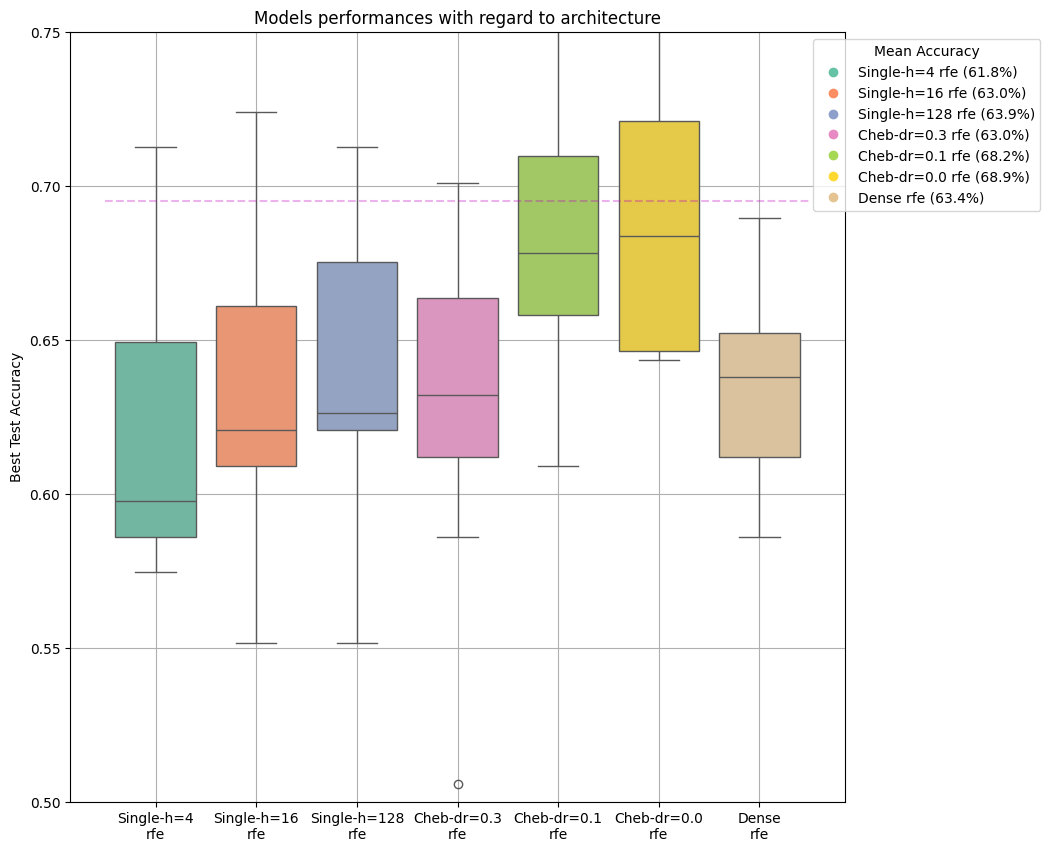
\includegraphics[width=0.45\textwidth]{figures/model_performances_architecture.png}
    \caption{Classification accuracy: comparison of different architectures.
    Single architectures are composed of a single hidden layer with a given number of neurons $h$.
    \textit{Dense} architecture refer to a fully connected neural network with a single hidden layer.
    \textit{Cheb} architectures refer to the graph convolution architecture, we vary the dropout rate $dr$
    during training.}
    \Description{}
    \label{fig:results_architecture}
\end{figure}

\begin{table}[H]
	\begin{center}
		\begin{tabular}{lll}
			Model & Feature & Test accuracy \\
			\hline
			Single-h=4 & rfe & 61.8 +/- 4.4\% \\
			Single-h=16 & rfe & 63.0 +/- 5.1\% \\
			Single-h=128 & rfe & 63.9 +/- 4.6\% \\
			Cheb-dr=0.3 & rfe & 63.0 +/- 5.4\% \\
			Cheb-dr=0.1 & rfe & 68.2 +/- 4.0\% \\
			Cheb-dr=0.0 & rfe & 68.9 +/- 4.0\% \\
			Dense & rfe & 63.4 +/- 3.3\% \\
		\end{tabular}
	\end{center}
	\caption{Models performances with regard to architecture}
	\label{table:dependance_on_architecture}
\end{table}


\subsection{Result on reduced features}

\subsection{Main limitations}


One prominent challenge that emerged from our experiments was the significant mismatch between the number of subjects ($871$) and the number of features (higher than $6100$), even after dimension reduction techniques were applied. This scenario places us squarely in the realm of the "curse of dimensionality," introducing complexities that can adversely impact the training of neural network models. With a limited number of subjects, the data points within the high-dimensional feature space become sparsely distributed. This sparsity poses challenges for neural networks, as they may struggle to capture meaningful patterns and relationships in the data, leading to overfitting or suboptimal generalization.

In particular, all the models were overfitting the training data, as evidenced by the large gap between the training and validation accuracies. We attempted to mitigate this issue by applying dropout and $L_2$ regularization. \blue{We note that the ChebGCN with a dropout rate of $0.1$ yields the best performance on the validation data}

In conclusion, our experiments encompassed a range of configurations, each designed to explore different facets of the model. Despite the diversity in hyperparameters and settings, the performance across these configurations on the test data exhibited minimal variations.